\section{WF+DNS attacks}
\label{sec:attack}
We begin by summarizing our attack.  Our attack is based on traffic correlation,
so it requires an attacker to observe traffic that is both entering and exiting
the Tor network.  In contrast to earlier work, we consider DNS instead of just
end-to-end TCP packets.
Our attack is illustrated in Figure~\ref{fig:attack-scenario} and requires the
following building blocks:
\begin{figure}[t]
	\centering
	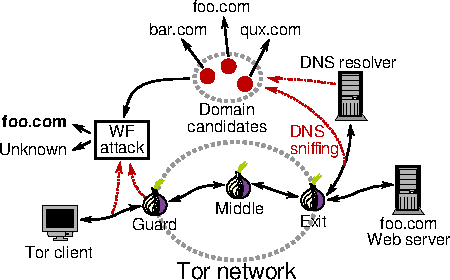
\includegraphics[width=0.8\linewidth]{figures/attack-scenario.pdf}
	\caption{An overview of our correlation attack.  An adversary must monitor
		both ingress and egress traffic.  A network-level adversary between the
		client and its guard monitors ingress traffic.  The same adversary
		monitors egress traffic between the exit and a DNS server, or the DNS
		server itself.  Both ingress (encrypted Tor traffic) and egress (DNS
		requests) traffic then serve as input to a Website fingerprinting
		attack.}
	\label{fig:attack-scenario}
\end{figure}

\begin{itemize}
    \item \emph{Ingress sniffing:} An attacker must observe traffic that is
		entering the Tor network.  The attacker can operate on the network level,
		i.e., be a malicious ISP, or an intelligence agency.  In addition, the
		attacker can operate on the relay level, i.e., run a malicious Tor guard
		relay.  Note that in both cases, the attacker can only observe encrypted
		data.  Therefore, packet meta information such as packet lengths and
		directions serve as input to a website fingerprinting
		attack~\cite{Panchenko2016a}.
    \item \emph{Egress sniffing:} To observe both ends of the communication, an
		attacker must also observe egress DNS traffic.  We expect the adversary
		to operate on the network level, i.e., be on the path between exit relay
		and a DNS server.  Alternatively, the attacker can run a malicious DNS
		resolver or server.  Note that an attacker may also run an exit relay,
		but in that case she might as well do classical end-to-end correlation.
\end{itemize}
We combine a classical WF attack operating on traffic from ingress sniffing with
DNS traffic observed by egress sniffing, creating WF+DNS attacks. Our attacks
correlate the web\emph{sites} observed by the WF attack in ingress traffic with
the web\emph{sites} identified from DNS traffic. Next, we describe how we
simulate the DNS traffic from Tor exits, how we map DNS requests to websites,
and finally present our two WF+DNS attacks.

\subsection{Simulating Tor-exits' DNS traffic}
\label{sec:attack:sim}
To estimate the capability of an attacker, we need to investigate what
DNS data is observable for the attacker: that is, what DNS request are
emerging from Tor exit relays.

We cannot use real data because there are no logs of outgoing traffic
from Tor exit relays available to us and ethical considerations kept us
from trying to collect them (\eg by operating exit relays and recording
the outgoing traffic). We therefore opt to \emph{simulate} the DNS traffic
emerging from Tor exit relays.

\subsubsection{Website Popularity Distribution}
\label{sec:attack:pop}
First, we model \emph{what websites} are visited by Tor users.
Currently, there are about 173 million active
websites\footnote{\url{http://news.netcraft.com/archives/2016/07/19/july-2016-web-server-survey.html}}
in the world and the Alexa ranking gives insights into their popularity
based on the browsing behaviour of a sample of all internet users
\footnote{\url{https://support.alexa.com/hc/en-us/articles/200449744}}.
It has been shown that the popularity of a website follows a powerlaw
distribution based on the rank of the
website~\cite{DBLP:journals/network/MahantiCMAW13}. So
we fit a powerlaw distribution to the page view numbers of the Alexa top
\fixme{@bgre: the alpha value here does not match, and this subsubsection does
not reflect our manual fitting which is the default for all our figures except
 for Figure 9 (d), please fix)}
10\,000 websites\footnote{We used the python powerlaw package
		\url{https://github.com/jeffalstott/powerlaw} for fitting, the
		resulting powerlaw distribution had an $\alpha$ parameter of
		$1.10291152854$. Page view numbers as collected by Alexa ignore
		multiple visits by the same user on the same day, so the ranking
		might be slightly off for our purposes.} and use the result to
model which websites are visited by Tor users.
This might overestimate the popularity of higher-ranked websites because
Tor users might be visiting less popular websites, such as websites that
are censored in different parts of the world, more often than the
average internet users and we will discuss the implications of this for
our results later on.

\subsubsection{Page load frequency}
\label{sec:load-freq}
% phw's numbers extrapolated
Second, we determined how many websites Tor users visit in a certain time span.
We approximated this number by seting up an exit relay whose exit policy
included only ports 80 and 443, so our relay would only forward web traffic.  We
then used tshark to capture the timestamps of DNS requests---but no DNS
responses.  We made sure that our tshark filter did not capture packet payloads
or headers, so we were unable to learn what websites Tor users were visiting.
In addition, we patched tshark so it would log timestamps at a granularity of
five minutes.  Given the limited granularity, we feel safe to publish this
dataset.  For an ethical discussion of this experiment, refer to
Section~\ref{sec:ethics}.  We ran the experiment for approximately two weeks
from May 15, 2016 to May 31, 2016, which allowed us to determine the number of
DNS requests for 4,832 five minute intervals.  The time series is illustrated in
Figure~\ref{fig:dns-reqs}.

\begin{figure}[t]
	\centering
	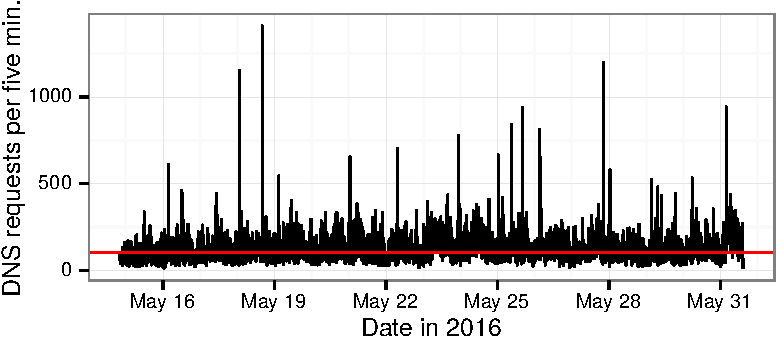
\includegraphics[width=\linewidth]{figures/dns-reqs.pdf}
	\caption{The number of DNS requests per five minute intervals on our
	exit relay.  Using a privacy-preserving measurement method, we only
	determined approximate timestamps and no content.  The red line at $y = 105$
	illustrates the median of the distribution.}
	\label{fig:dns-reqs}
\end{figure}

We then interpolate these numbers to all Tor exit relays based on the published
bandwidth statistics of all Tor exit relays. We found our exit relay to have on
average 119.3 outgoing DNS requests per 5 minutes during a two week period,
which corresponds to about 1.583 page visits per minute (taking caching into
\fixme{did this use the old powerlaw distribution?}
account and assuming a powerlaw distribution of site popularity as described
above).  The exit was configured to only allow port 80 and 443 during the time
of the measurements to avoid counting DNS requests from other protocols than
HTTP and HTTPS. We then used the self-reported bandwidth information from Tor
exit relays collected in the ``extra-info'' descriptors available on
CollecTor~\cite{collector} to estimate the number of page loads on each of the
about 1,200 exit relays active at that time.

\subsubsection{DNS caching}
To analyze which DNS requests can be seen by the adversary, we need to
take caching of DNS responses into account. We ignore client-side DNS
caching since it is disabled by default, as described in
Section~\ref{sec:background}.
% From Tobias: I manually could not get Firefox to cache anything,
% not even between pageloads on the same site (went to kau.se, waited 20s,
% then clicked on a link: little tor client-side still got a DNS response
% from the exit for kau.se.)
On the exit relays, where the actual DNS resolution takes place, caching
is highly relevant as the requests of all users connected to an exit
uses the same cache. An exit
relay maintains its own DNS cache\footnote{Around eventdns.c.  See the
		code in src/or/dns.c.} and enforces a minimum TTL of 60 seconds
and a maximum TTL of 30 minutes\footnote{See src/or/dns.c:278}.  We
refer to this as Tor's \emph{TTL clipping}. Due to a
bug\footnote{We redacted the link to the bug report to anonymize our paper
submission.}
% \url{https://bugs.torproject.org/19025}}
in Tor, the TTL of all DNS responses are set to 60 seconds.

%\subsubsection{Sliding window approach to compensate for DNS caching}
% we ignore caching by having a window of X minutes
If a user of an exit relay requests the IP address for a domain name
that has been cached by the exit relay before (and the cache entry is
not expired yet), then the adversary will not be able to observe an
outgoing DNS request for this domain name. But the adversary can
recorded all DNS requests from the exit relay in the past $x$ seconds,
where $x$ is the maximum TTL value (that is, maintain a sliding window of
length $x$) to obtain a list of all possibly requested domain names at the
given point in time. A domain name that is requested by a client at the
given point in time is either contained in the cache or not. If it is
not contained in the cache, it will be observable as a new, outgoing DNS
request from the exit relay. If it is contained in the cache it must
have been resolved by the exit relay in the last $x$ seconds and will
therefore be contained in the sliding window.

We assume that an adversary applies this sliding window technique and
model the observable DNS data accordingly.
The attacker observes a fraction of Tor exit bandwidth,
for a specific window length,
and together with our page load frequency estimation
this triggers a number of page loads in our simulation.
For each page load event we randomly draw a website using the
powerlaw website popularity distribution described above and put its
DNS requests into the window. As we will see next, we do not need to
simulate or consider the fact that the observed fraction of Tor exit bandwidth
corresponds to many different exits with individual caches.

\subsection{From DNS requests to websites}
Given a sliding window of DNS requests we investigate
how useful this information is in determining if websites of interest have
been visited or not. In April 2016 we visited Alexa top one million websites,
collecting five samples of all DNS requests generated by visiting each website.
Collection was done in rounds from our university network, where
each round uniformly randomly browsed all one million websites before visiting
the same website again. We used Tor Browser Bundle (TBB) 5.5.4
configured to \emph{not browse over Tor}: TBB ensures that the browser behavior
is  identical to a TBB user over Tor, and by not using Tor we bypass
IP-blacklists and CAPTCHAs triggered by IP-addresses of
Tor-exits~\cite{Khattak2016a}.
Table~\ref{tab:dns-censor} shows the percentage of websites in our dataset that
risks censorship by CloudFlare or Akami if collecting data over Tor, as
identified by Khattak et al.~\cite{Khattak2016a}. We also include Google, which
reportedly restricts access to Tor users (when searching), due to
their prevalance in the dataset.

\begin{table}[t]
	\centering
	\caption{The percentage of websites on Alexa top-one-million using providers
	involved in censoring or restricting access from Tor~\cite{Khattak2016a}.}
	\begin{tabular}{l r}
	\toprule
	\textbf{Description} & \textbf{Percentage} \\
	\midrule
	Website behind CloudFlare IP & 6.44 \\
	Domain on website uses CloudFlare & 25.81 \\
	Domain on website uses Akamai & 33.86 \\
	Domain on website uses Google & 77.43 \\
	\bottomrule
	\end{tabular}
	\label{tab:dns-censor}
\end{table}

We collected in total 2,540,941 distinct domain names over 60,828,453 DNS
requests. There are 2,260,534 \emph {unique domains} that are only requested on
a particular website. Figure~\ref{fig:unique-domains} shows the percentage of
sites with unique domains for different parts of Alexa top one million.
For 96.8\% of all sites there exists at least one uniqe domain, and the more
popular a site is the less likely it is to have a unique domain.
Table~\ref{tab:dns-requests} shows statistics for the number of DNS requests per
site. For at least half of the dataset we have ten requests per website where
two of them are unique.

\begin{figure}[t]
	\centering
	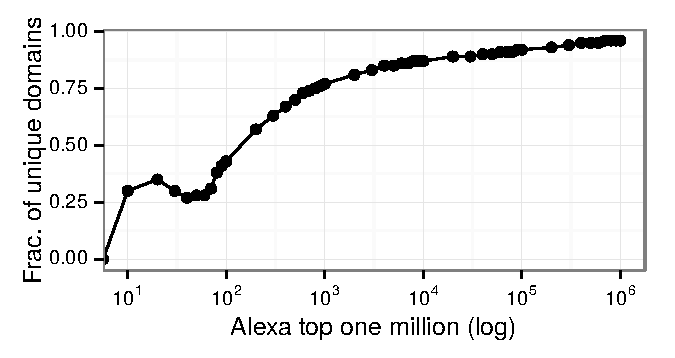
\includegraphics[width=0.7\linewidth]{figures/dns-unique-domains.pdf}
	\caption{The fraction of websites on Alexa top one million that has at least
	one unique domain. The vast majority of sites (96.8\%) have unique domains.}
	\label{fig:unique-domains}
\end{figure}

\begin{table}[t]
	\centering
	\caption{Statistics on the number of DNS requests.}
	\begin{tabular}{l r r r r}
	\toprule
	\textbf{DNS Requests} & \textbf{Median} & \textbf{Mean} & \textbf{Min} & \textbf{Max} \\
	\midrule
	per site & 10 & $12.2\pm11.2$ & 1 & 397 \\
	unique per site & 2 & $2.3\pm\phantom{0}1.8$ & 0 & 363 \\
	\bottomrule
	\end{tabular}
	\label{tab:dns-requests}
\end{table}

Table~\ref{tab:ttls} shows statistics on the TTL of DNS records in our dataset
for the TTL as-is (raw) and when clipped by Tor, for unique domains, and when
only considering the unique domain for each website with the lowest TTL.
Note that for about half of the websites on Alexa top one million, there is at
least one unique domain with a TTL of 60 seconds. Tor's TTL clipping has no
impact on the median TTL, but significantly influences the mean TTL.

\begin{table}[t]
\caption{Raw TTLs are unprocessed while Tor TTLs adhere to Tor's TTL clipping.
The unique prefix is for the TTL of unique domains while min unique only
considers the unique domains with the minimum TTL for each website.}
\centering
\begin{tabular}{l r r}
\toprule
\textbf{TTLs (s)} & \textbf{Median} & \textbf{Mean} \\
\midrule
% 2016/04/28 15:52:39 DNS records TTL mean 9780.0, std 42930.5, median 255.0, min 0.0, max 604800.0
raw & 255 & $9780.0\pm42930.5$ \\ % & 0 & 604800 \\
% 2016/04/28 15:44:05 DNS records TTL mean 701.5, std 755.3, median 255.0, min 60.0, max 1800.0
Tor & 255 & $701.5\pm\phantom{00}755.3$ \\ %& 60 & 1800 \\
% 2016/04/28 15:52:39 	unique domain TTL mean 13022.2, std 35054.4, median 900.0, min 0.0, max 604800.0
unique raw & 900 & $13022.2\pm35054.4$ \\ %& 0 & 604800 \\
% 2016/04/28 15:44:05 	unique domain TTL mean 1005.3, std 789.6, median 900.0, min 60.0, max 1800.0
unique Tor & 900 & $1005.3\pm\phantom{00}789.6$ \\ %& 60 & 1800 \\
% 2016/04/28 15:52:39 	unique domain _min_ TTL mean 3833.9, std 11073.6, median 60.0, min 0.0, max 604800.0
min unique raw & 60 & $3833.9\pm11073.6$ \\ % & 0 & 604800 \\
% 2016/04/28 15:44:05 	unique domain _min_ TTL mean 644.2, std 763.8, median 60.0, min 60.0, max 1800.0
min unique Tor & 60 & $644.2\pm\phantom{00}763.8$ \\ %& 60 & 1800 \\
\bottomrule
\end{tabular}
\label{tab:ttls}
\end{table}

To analyse the feasability of mapping DNS requests to websites we construct a
na\"{\i}ve website classifier: map each unique domain in a set of DNS requests
to the corresponding website.
With five-fold cross-validation on our Alexa top one million dataset with five
samples we consider a closed world and an open world: in the closed world the
attacker can use samples from all sites in training (as folded) while in the
open world some sites are unmonitored and therefore unknown (as per the fold).
In the closed world we get 0.970 recall and 0.994 precision.
For the open world we monitor Alexa top 500k and consider 369k unmonitored
sites. The number of unmonitored sites is extrapolated from our powerlaw
distribution, giving a relastic base rate (for the entire Tor network) for
evaluating our classifier.
In the open world we get 0.965 recall and 0.975 precision, slightly
worse than in the closed world.

Note that it is likely that website classification can be made
virtually perfect if accounting for order of requests, per-exit partitioning of
DNS requests, TTLs, and website popularity. The closed world setting
is also realistic when evaluating a classifier that maps DNS requests to
websites since gathering reuqets made by all 173 million active websites on the
Internet is practical with modest resources.
We use our conservative open world results when simulating the Tor network for
evaluating WF+DNS attacks but
highlight that our results indicate that observing DNS requests in Tor is
largely equivallent to observing sites visited over Tor.

\subsection{Our two WF+DNS attacks}
We use Wa-kNN by Wang et al.~\cite{Wang2014a} and a list of sites derived from
observing DNS requests for our two WF+DNS attacks:

\begin{description}
	\item[\texttt{ctw}] we ``close the world''
	on a modified Wa-kNN classifier by only considering the distance to observed
	sites when calculating the $k$-nearest neighbours. The classifier still
	considers the distance to all open instances to capture unmonitored sites.
	\item[\texttt{hp}] when Wa-kNN classifies a trace as a monitored site, confirm
	that we observed the same site in the DNS data (ensuring high precision). If
	not, make the final classification unmonitored.
\end{description}

Note that our approaches are generic and can be made to work with any WF attack
with little effort. The goal of the \texttt{ctw} attack is to move the WF attack
closer to a closed-world setting. Conceptually, the attack could also include
a custom weightlearning run---training only on observed sites---but our initial
results noted little to no gain at a significantly increases testing time.
This is probably because some features are just more useful than others
regardless of the training data~\cite{kfingerprinting}. The \texttt{hp} attack
is a straightforward (but highly effective) correlation attack: only produce
an output if both ingress and egress traffic are consistent.
